\documentclass[]{BasiliskReportMemo}
\usepackage{AVS}


\newcommand{\submiterInstitute}{Autonomous Vehicle Simulation (AVS) Laboratory,\\ University of Colorado}

\newcommand{\ModuleName}{test\textunderscore unitThrusterDynamics}
\newcommand{\subject}{Thruster Test}
\newcommand{\status}{Initial document}
\newcommand{\preparer}{S. Piggott}
\newcommand{\summary}{ This test compares the simulation's forces and torques due to thrusters with expected values. This test runs a variety of thrust scenarios, creates truth values, and compares them point by point to the simulation. It therefore analyses the thrust behavior down to test rate precision.}


\begin{document}


\makeCover



%
%	enter the revision documentation here
%	to add more lines, copy the table entry and the \hline, and paste after the current entry.
%
\pagestyle{empty}
{\renewcommand{\arraystretch}{2}
\noindent
\begin{longtable}{|p{0.5in}|p{4.5in}|p{1.14in}|}
\hline
{\bfseries Rev}: & {\bfseries Change Description} & {\bfseries By} \\
\hline
Draft & Initial Revision & T. Teil \\
\hline

\end{longtable}
}

\newpage
\setcounter{page}{1}
\pagestyle{fancy}

\tableofcontents
~\\ \hrule ~\\

%\begin{figure}[htb]
%	\centerline{
%	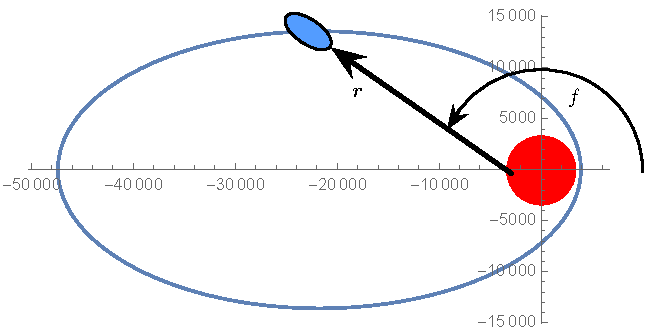
\includegraphics[]{Figures/Fig1}
%	}
%	\caption{Sample Figure Inclusion.}
%	\label{fig:Fig1}
%\end{figure}

\section{Introduction}
The Thruster model in the AVS Basilisk simulation is used to emulate the effect 
of a vehicle's thrusters on the overall system.  Its primary use is to generate 
realistic forces/torques on the vehicle structure and body.  This is 
accomplished by apply a force at a specified location/direction in the body and 
using the current vehicle center of mass to calculate the resultant torque.  
Each individual thruster in a given model has its own ramp-up/ramp-down profile 
specified as part of its initialization data and it follows those profiles during 
start-up and shutdown.

The thruster model also contains a mechanism that is used to change the current 
vehicle mass properties as the thruster fires propellant overboard.  This model 
uses the thruster ISP (specific impulse, also specified with configuration data) 
to calculate how much mass is being removed during a given thruster firing and 
decrements the mass properties included in the thruster linearly as a function 
of mass.  

The model can be configured according to the user's wishes, but the following 
rules of thumb should probably be respected unless you are incredibly confident 
in your own smartness.
\begin{enumerate}
\item{The internal simulation dynamics step time should be less than or equal 
     to the thruster ramp-up/ramp-down time steps}
\item{The internal simulation dynamics step time should be less than or equal to 
     the desired thruster discretization level}
\item{The internal simulation dynamics step time should be less than one-tenth 
    of the expected minimum allowable thruster firing duration}
\end{enumerate}


\section{Test Design}
The unit test for the thruster\_dynamics module is located in:\\

\noindent
{\tt SimCode/dynamics/Thrusters/$\_$UnitTest/unit$\_$ThrusterDynamicsUnit.py} \\
\\

The thruster parameters that were used are:

\begin{itemize}
\item The specific impulse: $I_{sp} = 266.7$s 

A thrusters potential to deliver force per mass flow rate. 
\item The maximum thrust: $F_{\mathrm{max}} = 1.0$ N

The scaling factor yielding the thrust.
\item The minimum On time: $t_{\mathrm{min}} = 0.006$s

The minimum time that the thruster can be fired.
\end{itemize}


\noindent This unit test is designed to functionally test the simulation model 
outputs as well as get complete code path coverage.  The test design is broken 
up into several parts:\\
\begin{enumerate}
\item{\underline{Instantaneous On/Off Factor:} The thrusters are fired with an 
  instantaneous ramp to ensure that the firing is correct. This gives us a base case.}
\item{\underline{Short Instantaneous Firing:} A "short" firing that still respects the 
  rules of thumb above is fired to ensure that it is still correct.}
 \item{\underline{Short Instantaneous Firing with faster test rate:} A "short" firing that still respects the 
  rules of thumb above but with a faster test rate to see the jump.}
 \item{\underline{Instantaneous On/Off Factor with faster test rate:} The thrusters are fired with an 
  instantaneous ramp to ensure that the firing is correct given a different test rate. This shouldn't modify the physics.}
 \item{\underline{Thruster Angle Test:} The output forces/torques from the simulation 
  are checked with a thruster pointing in a different direction.}
   \item{\underline{Thruster Position Test:} The output forces/torques from the simulation 
  are checked with a thruster in a different position.}
   \item{\underline{Thruster Number Test:} The output forces/torques from the simulation 
  are checked with two thruster in different positions, with different angles.}
\item{\underline{Ramp On/Ramp Off Firing:} A set of ramps are set for the thruster to ensure 
  that the ramp configuration is respected during a ramped firing.}
  \item{\underline{Short ramped firing:} A thruster is fired for less than the amount of time it 
   takes to reach the end of its ramp.}
\item{\underline{Ramp On/Ramp Off Firing with faster test rate:} A set of ramps are set for the thruster to ensure 
  that the ramp configuration is respected during a ramped firing with different test rate.}
\item{\underline{Cutoff firing:} A thruster is commanded off (zero firing time) in the middle 
   of its ramp up to ensure that it correctly cuts off the current firing}
\item{\underline{Ramp down firing:} A thruster is fired during the middle of its ramp down 
   to ensure that it picks up at that point in its ramp-up curve and reaches 
   steady state correctly.}
\end{enumerate}

\section{Truth Values}

In order to have a rigorous automated test, we have to predict the forces and torques that will apply on the spacecraft. We use the following equations to compute the thrust at each time step. We call $\alpha$ the angle in which the thruster is pointing, $\bm r = r \hat{\bm e_r}= \left(r_x, r_y, r_z \right)$ it's position vector, 

\begin{enumerate}
\item{\underline{With one thruster}}: The forces are simply the projections of the thrust force on the axes of interest. The torque along $x$ is the arm along $z$ times the projection of the force along $y$, the torque along $z$ is the arm along $x$ times the projection of the force along $y$, the torque along $z$ is the arm along $x$ times the projection of the force along $y$. 

\begin{align}
F_x =F_{\mathrm{max}} \cos \alpha &\hspace{1cm} T_x = - F_{\mathrm{max}}\sin(\alpha) r_z \\ 
F_y = F_{\mathrm{max}} \sin \alpha &\hspace{1cm} T_y = F_{\mathrm{max}} \cos(\alpha) r \sin( \arctan(r_z/r_x)) \\ 
F_z = 0 &\hspace{1cm} T_z =  F_{\mathrm{max}} \sin(\alpha) r_x 
\end{align}


\item{\underline{With two thrusters}}: By giving indices $1$ and $2$ for each of the thrusters, we just need to add the Forces and torques defined above to get the total Forces and Torques:

\begin{align}
F_x = F_{x1} + F_{x2} &\hspace{1cm} T_x = T_{x1} + T_{x2} \\ 
F_y =  F_{y1} + F_{y2} &\hspace{1cm} T_y =  T_{y1} + T_{y2}\\ 
F_z =  F_{z1} + F_{z2} &\hspace{1cm} T_z =  T_{z1} + T_{z2}
\end{align}

\item{\underline{With ramps thruster}}: When the thrusters now ramp up and down, we create a normalized ramp function $\rho$. An example is given in \ref{fig:Ramp_function} in the case of a cutoff fire and renewed fire. \par

 \input{AutoTex/Ramp_function.tex}

We then prolong the force and torque end times as a function of the ramp slope, and multiply the inital functions by this ramping function:

\begin{align}
\tilde{F_x} = \rho F_{x} &\hspace{1cm} \tilde{T_x} =\rho T_{x}  \\ 
\tilde{F_y} =  \rho F_{y}  &\hspace{1cm} \tilde{T_y} =\rho  T_{y} \\ 
\tilde{F_z} = \rho F_{z} &\hspace{1cm} \tilde{T_z} =\rho  T_{z} 
\end{align}

\end{enumerate}

\section{Test Results}

\begin{enumerate}
\item{\underline{ Instantaneous On/Off Factor}:} 

\input{AutoTex/Snippet1Thrusters_5s_30deg_Loc2_Rate10.tex}

 Figures \ref{fig:Force_1Thrusters_5s_30deg_Loc2_Rate10} and \ref{fig:Torque_1Thrusters_5s_30deg_Loc2_Rate10} show the force and torque behaviors (respectfully) for the thruster unit test.
    
    \input{AutoTex/Force_1Thrusters_5s_30deg_Loc2_Rate10.tex}
    \input{AutoTex/Torque_1Thrusters_5s_30deg_Loc2_Rate10.tex}
    \input{AutoTex/1Thrusters_5s_30deg_Loc2_Rate10.tex}
    
    As Figure \ref{fig:1Thrusters_5s_30deg_Loc2_Rate10} shows, the desired behavior is captured exactly for each 
    firing in the test for all of the forces and torques. This is validated by the exact same predicted and simulated thrust arrays.  \textcolor{ForestGreen}{Test successful.}

\item{\underline{Short Instantaneous Firing: }}

\input{AutoTex/Snippet1Thrusters_0s_30deg_Loc2_Rate10.tex}

 Figure \ref{fig:Force_1Thrusters_0s_30deg_Loc2_Rate10} shows the force behavior given this short input. We see that the test rate begin small next to the thrust duration, doesn't capture the jump quite well.
    
    \input{AutoTex/Force_1Thrusters_0s_30deg_Loc2_Rate10.tex}
    \input{AutoTex/1Thrusters_0s_30deg_Loc2_Rate10.tex}
    
    As Figure \ref{fig:1Thrusters_0s_30deg_Loc2_Rate10} shows, the desired behavior is captured exactly for each 
    firing in the test for all of the forces and torques. Despite the lower test rate, the forces and torques behave appropriately. This is validated by the exact same predicted and simulated thrust arrays.\textcolor{ForestGreen}{Test successful.}

 \item{\underline{Short Instantaneous Firing with faster test rate: }}
 
 \input{AutoTex/Snippet1Thrusters_0s_30deg_Loc2_Rate1000.tex}

 Figure \ref{fig:Force_1Thrusters_0s_30deg_Loc2_Rate1000} shows the force behavior given the same short input as previously. We now see that the jump is well resolved.
    
    \input{AutoTex/Force_1Thrusters_0s_30deg_Loc2_Rate1000.tex}
    \input{AutoTex/1Thrusters_0s_30deg_Loc2_Rate1000.tex}
    
    As Figure \ref{fig:1Thrusters_0s_30deg_Loc2_Rate1000} shows, the desired behavior is captured exactly for each 
    firing in the test for all of the forces and torques. This is validated by the exact same predicted and simulated thrust arrays. \textcolor{ForestGreen}{Test successful.}
 
 \item{\underline{Instantaneous On/Off Factor with faster test rate:} }
 
  \input{AutoTex/Snippet1Thrusters_5s_30deg_Loc2_Rate100.tex}

 The thrust command given is now 5 seconds long, as in the base test. The difference is that the test rate is now augmented in order to guarantee that it does not affect the test.
     
    \input{AutoTex/1Thrusters_5s_30deg_Loc2_Rate100.tex}
    
    As Figure \ref{fig:1Thrusters_5s_30deg_Loc2_Rate100} shows, the desired behavior is captured exactly for each 
    firing in the test for all of the forces and torques. This is validated by the exact same predicted and simulated thrust arrays. \textcolor{ForestGreen}{Test successful.}
 
 \item{\underline{Thruster Angle Test:}}
 
   \input{AutoTex/Snippet1Thrusters_5s_10deg_Loc2_Rate10.tex}

 The test now shows that the simulation still behaves with different thruster orientations.
     
    \input{AutoTex/1Thrusters_5s_10deg_Loc2_Rate10.tex}
    
    As Figure \ref{fig:1Thrusters_5s_10deg_Loc2_Rate10} shows, the desired behavior is captured exactly for each 
    firing in the test for all of the forces and torques. This is validated by the exact same predicted and simulated thrust arrays. \textcolor{ForestGreen}{Test successful.}
 
 
   \item{\underline{Thruster Position Test:} }
   
      \input{AutoTex/Snippet1Thrusters_5s_30deg_Loc0_Rate10.tex}

 This test shows that different locations still give correct values for forces and torques.
      
    \input{AutoTex/1Thrusters_5s_30deg_Loc0_Rate10.tex}
    
    As Figure \ref{fig:1Thrusters_5s_30deg_Loc0_Rate10} shows, the desired behavior is captured exactly for each 
    firing in the test for all of the forces and torques. This is validated by the exact same predicted and simulated thrust arrays. \textcolor{ForestGreen}{Test successful.}
   
   \item{\underline{Thruster Number Test:} }
   
         \input{AutoTex/Snippet2Thrusters_5s_30deg_Loc2_Rate10.tex}

 This test shows that the thruster model can incorporate several thrusters correctly. We add a second thruster and use the modified truth function for the forces and torques.
      
    \input{AutoTex/2Thrusters_5s_30deg_Loc2_Rate10.tex}
    
    As Figure \ref{fig:2Thrusters_5s_30deg_Loc2_Rate10} shows, the desired behavior is captured exactly for each 
    firing in the test for all of the forces and torques. This is validated by the exact same predicted and simulated thrust arrays.  \textcolor{ForestGreen}{Test successful.}
   
\item{\underline{Ramp On/Ramp Off Firing:} }

         \input{AutoTex/SnippetRamp_10steps_5s_CutoffOFF_Rate10_CutoffOFF.tex}

 This test now ramps the thrust up and down. We use a 10 step ramp that takes $0.1$s to climb and fall. This ramp time is slightly exaggerated in order to see the ramp clearly.      
    \input{AutoTex/Ramp_10steps_CutoffOFF_5s_testRate10.tex}
    
    As Figure \ref{fig:Ramp_10steps_CutoffOFF_5s_testRate10} shows, the desired behavior is captured exactly for each 
    firing in the test for all of the forces and torques. This is validated by the exact same predicted and simulated thrust arrays. \textcolor{ForestGreen}{Test successful.}
   

  \item{\underline{Short ramped firing:} }
  
    \input{AutoTex/SnippetRamp_10steps_0s_CutoffOFF_Rate10_CutoffOFF.tex}

Using the same ramp, the thruster fires for $0.5$s. We expect to see a climb and immediate fall of the thrust factor.
       
    \input{AutoTex/Ramp_10steps_CutoffOFF_0s_testRate10.tex}
    
    As Figure \ref{fig:Ramp_10steps_CutoffOFF_0s_testRate10} shows, the desired behavior is captured exactly for each 
    firing in the test for all of the forces and torques. This is validated by the exact same predicted and simulated thrust arrays. \textcolor{ForestGreen}{Test successful.}
  
\item{\underline{Ramp On/Ramp Off Firing with faster test rate:} }

    \input{AutoTex/SnippetRamp_10steps_5s_CutoffOFF_Rate100_CutoffOFF.tex}

 Using once again the same ramp, we run the test for $5$ seconds with a faster test rate. We seek to validate that the test rate has no impact on the simulation.
      
    \input{AutoTex/Ramp_10steps_CutoffOFF_5s_testRate100.tex}
    
    As Figure \ref{fig:Ramp_10steps_CutoffOFF_5s_testRate100} shows, the desired behavior is captured exactly for each 
    firing in the test for all of the forces and torques. This is validated by the exact same predicted and simulated thrust arrays. \textcolor{ForestGreen}{Test successful.}

\item{\underline{Cutoff firing:}}

 \input{AutoTex/SnippetRamp_10steps_CutoffON_Rate10_CutoffON.tex}

 Using the same ramp, we start firing the thruster with an initial command of 5 seconds. After just $0.2$ seconds of thrust ramping, we change the test command and thrust for $0.3$ seconds. This leads to a total thrust of $0.5$ seconds, and validates the fact that the command was properly overridden.
      
    \input{AutoTex/Ramp_10steps_CutoffON_5s_testRate10.tex}
    
    As Figure \ref{fig:Ramp_10steps_CutoffON_5s_testRate10} shows, the desired behavior is captured exactly for each 
    firing in the test for all of the forces and torques. This is validated by the exact same predicted and simulated thrust arrays. \textcolor{ForestGreen}{Test successful.}

\item{\underline{Ramp down firing:}}

 \input{AutoTex/SnippetRamp_10steps_CutoffON_Rate10rampDownON.tex}

 In this test, the initial command is of $0.5$ seconds. On the falling side of the ramp, a new command is given for $1.5$s. We expect to see the thrust climb again to steady state and last for the expected command time.   
      
    \input{AutoTex/Ramp_10steps_CutoffONrampDownON_testRate10.tex}
    
    As Figure \ref{fig:Ramp_10steps_CutoffONrampDownON_testRate10} shows, the desired behavior is captured exactly for each 
    firing in the test for all of the forces and torques. This is validated by the exact same predicted and simulated thrust arrays.  \textcolor{ForestGreen}{Test successful.}

\end{enumerate}




\section{Test Coverage}
The method coverage for all of the methods included in the spice\_interface 
module are tabulated in Table~\ref{tab:cov_met}

\begin{table}[htbp]
    \caption{Test Analysis Results}
   \label{tab:cov_met}
        \centering \fontsize{10}{10}\selectfont
   \begin{tabular}{c | r | r | r} % Column formatting, 
      \hline
      Method Name    & Unit Test Coverage (\%) & Runtime Self (\%) & Runtime Children (\%) \\
      \hline
      SelfInit & 100.0 & 0.0 & 0.0 \\
      CrossInit & 100.0 & 0.0 & 0.0 \\
      AddThruster & 100.0 & 0.0 & 0.0 \\
      UpdateState & 100.0 & 0.0 & 0.0 \\
      WriteOutputMessages & 100.0 & 0.0 & 0.0 \\
      ReadInputs & 100.0 & 0.0 & 0.0 \\
      ConfigureThrustRequests & 100.0 & 0.0 & 0.0 \\
      ComputeDynamics & 100.0 & 0.0 & 9.8 \\
      ComputeThrusterFire & 100.0 & 0.0 & 0.0 \\
      ComputeThrusterShut & 100.0 & 0.0 & 0.0 \\
      updateMassProperties & 100.0 & 0.0 & 0.6 \\
      \hline
   \end{tabular}
\end{table}

For all of the methods in the spice\_interface modules, the code coverage 
percentage is 100\% which meets our test requirements.  Additionally, 100\% of 
all code branches in the thruster\_dynamics source code were executed by this 
test.

%The test that was run to calculate thruster CPU usage was deliberately selected as 
%a stressing case for the thruster model.  The MOI burn was executed 9000 seconds 
%after the simulation was initialized and that maneuver takes 2000 seconds, so 
%approximately 20\% of the simulation was run with the vehicle under thrust.  
%With this stressing case, the ThrusterDynamics model accounted for 10\% of the 
%overall processing, which is certainly acceptable at this time.

The main CPU usage of the thruster\_dynamics source code occurs in the 
ComputeDynamics method that is called by the dynamics source.  The 
ThrusterDynamics methods themselves account for very little of the processing 
and it is the vector/matrix manipulation utilities called from the source that 
are the main culprits.  While the thruster model's ComputeDynamics function is 
using 50\% of the dynamics processing, that is only amounting to 10\% of the 
overall simulation processing.  The rest of the architecture in Basilisk should 
allow us to take the processing hit that we are getting from the 
ThrusterDynamics module without issue.

\section{Conclusions}
The thruster module has sufficient fidelity to accomplish the analysis 
that we need to perform thrust maneuvers.  All model capabilities were 
tested and analyzed in this document with all observed performance being nominal 
compared to the going-in expectation. Every line of source code was successfully tested and the integrated model 
performance was analyzed and is acceptable. Furthermore many thrust scenarios were tested in order to cover all outcomes of a maneuver and the robustness of the simulation.

% There are small updates that could 
%be made to get a slight performance increase if necessary, but the work that 
%would be required to get that performance bump does not seem worthwhile at this 
%time especially since the vehicle (and all spacecraft) spends so little of its 
%time under thrust.

\end{document}
